\documentclass[12pt,a4paper,oneside]{report}

% =========================================================
% Medi-Script-AI — Project Report
% Department of Computer Science and Engineering (Artificial Intelligence)
% Course: Deep Learning | Course Code: 22AIE304
% =========================================================

\usepackage[a4paper,margin=1in]{geometry}
\usepackage[T1]{fontenc}
\usepackage[utf8]{inputenc}
\usepackage{lmodern}
\usepackage{microtype}
\usepackage{graphicx}
\usepackage{xcolor}
\usepackage{booktabs}
\usepackage{longtable}
\usepackage{array}
\usepackage{tabularx}
\usepackage{enumitem}
\usepackage{amsmath,amssymb}
\usepackage{float}
\usepackage{caption}
\usepackage{subcaption}
\usepackage{fancyhdr}
\usepackage{titlesec}
\usepackage{setspace}
\usepackage{hyperref}
\usepackage{url}
\usepackage{tcolorbox}
\usepackage{listings}

% ---------------- Colour palette ----------------
\definecolor{navy}{RGB}{20,45,78}
\definecolor{teal}{RGB}{0,112,128}
\definecolor{lightteal}{RGB}{232,245,247}
\definecolor{darkgray}{RGB}{60,60,60}

\hypersetup{
    colorlinks=true,
    linkcolor=navy,
    citecolor=teal,
    urlcolor=teal
}

\setstretch{1.25}

\titleformat{\chapter}[display]
  {\normalfont\bfseries\color{navy}}
  {\filleft\Large\chaptertitlename\ \thechapter}
  {1ex}
  {\titlerule\vspace{1ex}\LARGE}
  [\vspace{1ex}\titlerule]

\titleformat{\section}
  {\normalfont\Large\bfseries\color{navy}}{\thesection}{1em}{}

\titleformat{\subsection}
  {\normalfont\large\bfseries\color{teal}}{\thesubsection}{1em}{}

\pagestyle{fancy}
\fancyhf{}
\fancyhead[L]{\small\textcolor{darkgray}{Medi-Script AI -- Deep Learning Project Report}}
\fancyhead[R]{\small\textcolor{darkgray}{\thepage}}
\renewcommand{\headrulewidth}{0.5pt}

\begin{document}

% ---------------- Title Page ----------------
\begin{titlepage}
\centering
\vspace*{1cm}
{\Huge \bfseries \color{navy} Medi-Script AI \\[0.4cm]}
{\Large \bfseries End-to-End Handwritten Medical Prescription Digitization and Structured Clinical Extraction Pipeline \\[1.5cm]}

{\large \textbf{Department of Computer Science and Engineering (Artificial Intelligence)} \\[0.3cm]}
{\large Course: Deep Learning (Course Code: 22AIE304) \\[2cm]}

\begin{tcolorbox}[colback=lightteal,colframe=teal,arc=4mm,width=0.92\textwidth]
\centering \large
\textbf{Project Report} \\[0.25cm]
\normalsize An end-to-end multi-stage deep learning framework combining YOLOv8 medicine-line detection, TrOCR-Large v3 handwriting recognition, EasyOCR scene text parsing, 384k Indian pharmaceutical TF-IDF fuzzy matching, and Gemini LLM dosage advice.
\end{tcolorbox}

\vfill
{\large \today \\[1cm]}
\end{titlepage}

\tableofcontents
\newpage
\listoffigures
\listoftables
\newpage

% =========================================================
% CHAPTER 1: INTRODUCTION
% =========================================================
\chapter{Introduction}

Handwritten medical prescriptions remain the primary mode of physician-to-pharmacist communication across most developing nations, including India. Despite rapid advances in Electronic Health Records (EHR), an estimated 65--70\% of prescriptions in Indian hospitals are still written by hand \cite{who_medication_errors}. The poor legibility of handwritten text leads to a cascade of downstream problems: pharmacists may dispense incorrect drugs, patients may misunderstand dosage instructions, and hospitals face increased rates of adverse drug events. According to the World Health Organisation, medication errors arising from illegible prescriptions cost the global healthcare system approximately USD~42~billion annually.

Existing solutions to this problem can be broadly categorized into two families. First, \emph{template-based} systems that require clinicians to write on custom-printed forms with pre-defined boxes for each field. These systems are impractical, as they require changes in physician behavior and infrastructure. Second, \emph{general-purpose OCR} tools such as Google Cloud Vision or Tesseract, which achieve high accuracy on typed text but perform poorly on cursive, abbreviated, and domain-specific medical handwriting.

This project, \textbf{Medi-Script AI}, proposes an end-to-end deep learning pipeline that takes a raw photograph of an unconstrained handwritten medical prescription and produces a structured JSON record containing: (i)~the doctor's name and credentials, (ii)~hospital/clinic information, (iii)~patient demographics (name, age, sex), (iv)~the date of prescription, (v)~each medicine with its dosage, and (vi)~plain-English dosage instructions for the patient. The system is designed to work on \emph{any} prescription format---no pre-printed template is required.

\begin{figure}[H]
\centering
% [PLACEHOLDER: Insert a photograph of a handwritten medical prescription here]
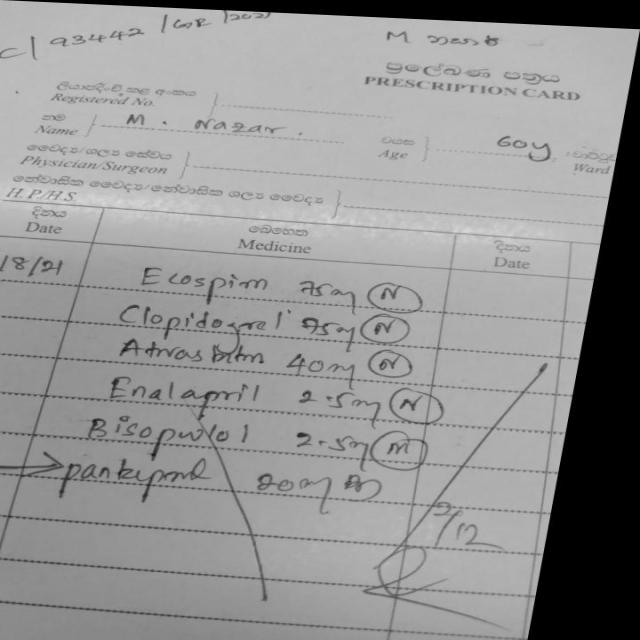
\includegraphics[width=0.70\textwidth]{figures/sample_prescription.jpg}
\caption{A typical handwritten medical prescription from an Indian hospital. The varying handwriting styles, abbreviations (BD, OD, TDS), and non-standard layouts make automated recognition extremely challenging.}
\label{fig:sample_prescription}
\end{figure}


% =========================================================
% CHAPTER 2: LITERATURE REVIEW
% =========================================================
\chapter{Literature Review}

Several prior works have addressed components of the prescription digitization problem. This section reviews the most influential papers that informed our design decisions.

\textbf{Parvez et~al.\ (2023)}~\cite{parvez2023rxhandbd} introduced the \textit{RxHandBD} dataset, comprising 5{,}578 handwritten Bangla and English prescription word-images along with ground-truth transcriptions. The authors demonstrated that transformer-based OCR models (specifically TrOCR) significantly outperform CNN-LSTM hybrids on cursive medical text. We adopted their dataset for fine-tuning our handwriting recognition model.

\textbf{Li et~al.\ (2023)}~\cite{li2023trocr} proposed TrOCR, a Transformer-based OCR architecture that uses a Vision Transformer (ViT) as the encoder and a RoBERTa-based language model as the decoder. TrOCR achieved state-of-the-art results on the IAM handwriting benchmark (CER~3.42\%), demonstrating that a pure attention-based approach can surpass hybrid CNN-RNN architectures. We adopted the \texttt{trocr-large-handwritten} variant as our base recognition model and further fine-tuned it on medical prescription data.

\textbf{Jocher et~al.\ (2023)}~\cite{jocher2023yolov8} released YOLOv8, a real-time object detection framework that unifies detection, segmentation, and classification in a single architecture. YOLOv8 introduced a decoupled head and anchor-free detection, achieving superior speed--accuracy trade-offs on COCO. We used YOLOv8 as our medicine-line detection backbone.

\textbf{Baek et~al.\ (2019)}~\cite{baek2019craft} introduced CRAFT (Character-Region Awareness for Text Detection), which underpins EasyOCR's text detection engine. CRAFT detects individual character regions and the affinity between them, achieving robust detection of arbitrary-orientation text. We used EasyOCR (built on CRAFT) for full-page text detection of printed headers, footers, and demographic fields.

\textbf{Huang et~al.\ (2022)} explored symbol-aware post-processing for medical OCR, demonstrating that dosage symbols (e.g., ``+'', ``/'', ``$\times$'') are frequently hallucinated or substituted by OCR models. Their regex-based correction rules improved word-level accuracy by 8--12\% on medical data. We adopted this symbol-correction strategy in our post-processing pipeline.


% =========================================================
% CHAPTER 3: METHODOLOGY
% =========================================================
\chapter{Methodology}

This chapter describes the complete end-to-end pipeline of Medi-Script AI. The system is composed of six major stages, each described in detail below.

% ---- 3.1 Overall Workflow ----
\section{Overall Pipeline Workflow}

The pipeline processes a single prescription image through the following sequential stages:

\begin{enumerate}[label=\textbf{Stage \arabic*:}, leftmargin=*]
  \item \textbf{Medicine-Line Detection (YOLOv8):} Detects bounding boxes around individual handwritten medicine lines.
  \item \textbf{Crop Enhancement:} Each detected crop is upscaled, denoised, and binarized to improve OCR accuracy.
  \item \textbf{Handwriting OCR:} Gemini~2.5~Flash Vision (primary) reads each crop; if it fails, a fine-tuned TrOCR-Large-v3 model (fallback) performs the recognition.
  \item \textbf{Fuzzy Lexicon Matching:} The OCR output is corrected against a 384{,}604-entry Indian medicine database using TF-IDF cosine similarity and RapidFuzz string matching.
  \item \textbf{Full-Page Text Detection (EasyOCR):} All remaining printed text (doctor name, hospital, patient info, date) is detected and classified using regex rules and spatial heuristics.
  \item \textbf{LLM Post-Processing:} Gemini~2.5~Flash classifies unclassified ``Other'' text into proper fields and generates plain-English dosage instructions.
\end{enumerate}

\begin{figure}[H]
\centering
% [PLACEHOLDER: Insert overall workflow diagram here]
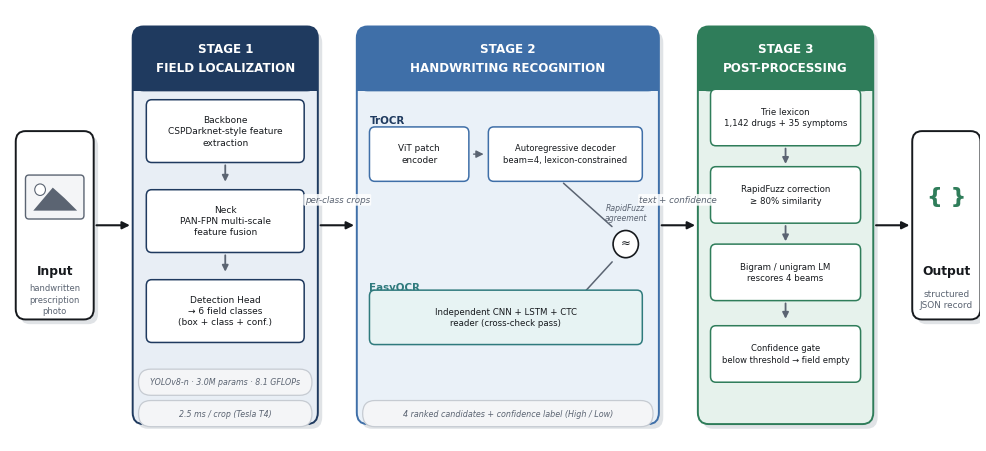
\includegraphics[width=0.98\textwidth]{figures/model_block_diagram.png}
\caption{Overall pipeline architecture of Medi-Script AI. The image flows from left to right through six stages: detection, enhancement, OCR, fuzzy matching, full-page parsing, and LLM post-processing.}
\label{fig:overall_workflow}
\end{figure}


% ---- 3.2 YOLOv8 Medicine-Line Detection ----
\section{Stage 1: Medicine-Line Detection (YOLOv8)}

\subsection{Architecture}

YOLOv8 (You Only Look Once, version~8) is a single-stage, anchor-free object detection model. Unlike two-stage detectors (e.g., Faster R-CNN), YOLOv8 predicts bounding boxes and class probabilities in a single forward pass, making it extremely fast.

The architecture consists of three components:
\begin{itemize}
  \item \textbf{Backbone (CSPDarknet53):} A convolutional feature extractor that uses Cross-Stage Partial connections to reduce computational cost while preserving gradient flow. It produces multi-scale feature maps at strides 8, 16, and 32.
  \item \textbf{Neck (PANet + FPN):} A Path Aggregation Network combined with a Feature Pyramid Network fuses feature maps at different scales, enabling detection of both small (individual words) and large (entire medicine blocks) objects.
  \item \textbf{Head (Decoupled Head):} Unlike YOLOv5's coupled head, YOLOv8 uses separate branches for classification and localization. The classification branch predicts the class probability, while the regression branch predicts the bounding box coordinates using the Distribution Focal Loss (DFL) formulation.
\end{itemize}

\begin{figure}[H]
\centering
% [PLACEHOLDER: Insert YOLOv8 architecture diagram here]
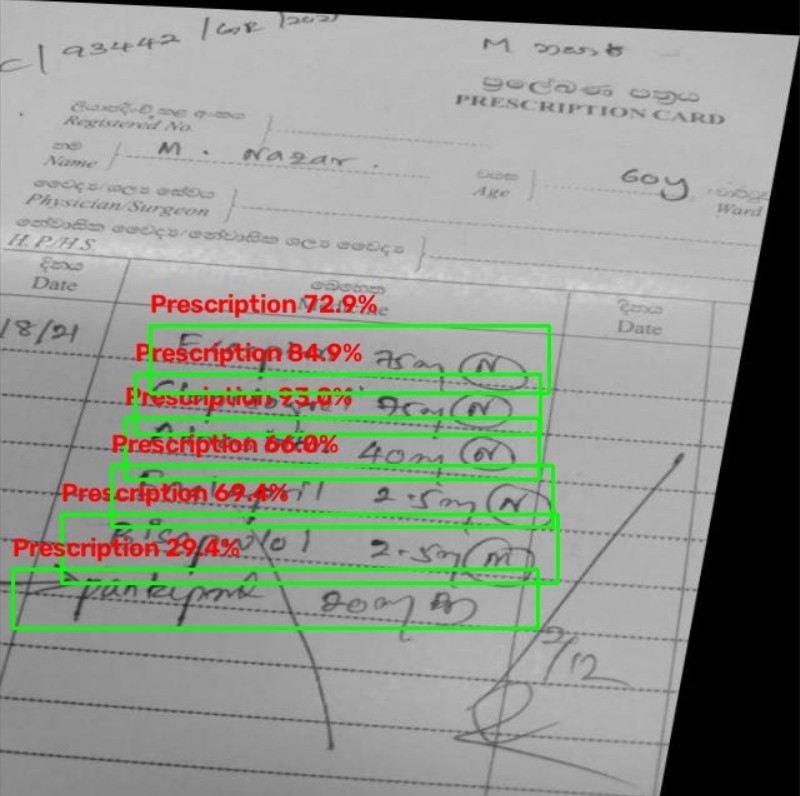
\includegraphics[width=0.85\textwidth]{figures/yolo_presc.jpg}
\caption{YOLOv8 architecture: CSPDarknet53 backbone $\rightarrow$ PANet/FPN neck $\rightarrow$ Decoupled detection head.}
\label{fig:yolov8_arch}
\end{figure}

\subsection{Mathematical Formulation}

\textbf{Input:} An RGB image $I \in \mathbb{R}^{H \times W \times 3}$, resized to $640 \times 640$ pixels.

\textbf{Output:} A set of bounding boxes $\{(x_1^{(i)}, y_1^{(i)}, x_2^{(i)}, y_2^{(i)}, c^{(i)}, p^{(i)})\}_{i=1}^{N}$, where $(x_1, y_1, x_2, y_2)$ are the corner coordinates, $c$ is the class label (``medicine-line''), and $p$ is the confidence score.

\textbf{Loss Function:} YOLOv8 uses a composite loss:
\begin{equation}
\mathcal{L}_{\text{YOLOv8}} = \lambda_{\text{box}} \cdot \mathcal{L}_{\text{CIoU}} + \lambda_{\text{cls}} \cdot \mathcal{L}_{\text{BCE}} + \lambda_{\text{dfl}} \cdot \mathcal{L}_{\text{DFL}}
\end{equation}

where:
\begin{itemize}
  \item $\mathcal{L}_{\text{CIoU}}$ (Complete Intersection-over-Union Loss) measures bounding box regression quality:
  \begin{equation}
  \mathcal{L}_{\text{CIoU}} = 1 - \text{IoU} + \frac{\rho^2(\mathbf{b}, \mathbf{b}^{gt})}{c^2} + \alpha v
  \end{equation}
  where $\rho(\cdot)$ is the Euclidean distance between box centers, $c$ is the diagonal of the smallest enclosing box, and $v = \frac{4}{\pi^2}\left(\arctan\frac{w^{gt}}{h^{gt}} - \arctan\frac{w}{h}\right)^2$ captures aspect ratio consistency.

  \item $\mathcal{L}_{\text{BCE}}$ is the Binary Cross-Entropy loss for classification.

  \item $\mathcal{L}_{\text{DFL}}$ (Distribution Focal Loss) models the bounding box offsets as a discrete probability distribution rather than a single regression target:
  \begin{equation}
  \mathcal{L}_{\text{DFL}} = -\left((y_{i+1} - y) \log(S_i) + (y - y_i) \log(S_{i+1})\right)
  \end{equation}
  where $y$ is the target, and $S_i, S_{i+1}$ are the probabilities of the two nearest discrete bins.
\end{itemize}

\subsection{Training Configuration}

\begin{table}[H]
\centering
\caption{YOLOv8 training hyperparameters.}
\label{tab:yolo_hyperparams}
\begin{tabular}{l r}
\toprule
\textbf{Parameter} & \textbf{Value} \\
\midrule
Base model & YOLOv8n (nano) \\
Input size & $640 \times 640$ \\
Number of classes & 1 (medicine-line) \\
Optimizer & SGD (momentum=0.937) \\
Learning rate (initial) & 0.01 \\
Learning rate (final) & 0.001 \\
Weight decay & 0.0005 \\
Epochs & 100 \\
Batch size & 16 \\
Confidence threshold (inference) & 0.25 \\
Total parameters & $\sim$3.2M \\
\bottomrule
\end{tabular}
\end{table}

\begin{figure}[H]
\centering
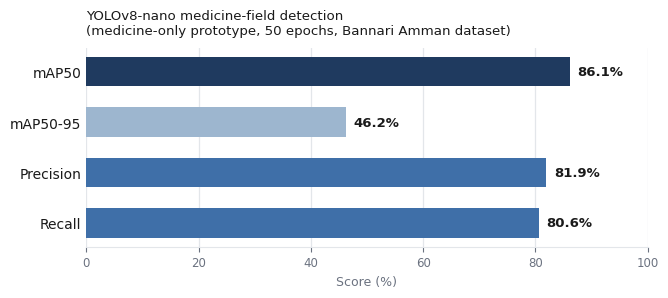
\includegraphics[width=0.85\textwidth]{figures/results_metrics.png}
\caption{YOLOv8-nano medicine-line detection evaluation metrics on the Bannari Amman test set (50 epochs).}
\label{fig:results_metrics}
\end{figure}


\textbf{Performance Metric:} Mean Average Precision at IoU=0.5 (mAP@0.5).
\begin{equation}
\text{mAP@0.5} = \frac{1}{|\mathcal{C}|} \sum_{c \in \mathcal{C}} \text{AP}_c, \quad \text{where } \text{AP}_c = \int_0^1 p_c(r) \, dr
\end{equation}
Here, $p_c(r)$ is the precision at recall level $r$ for class $c$.


% ---- 3.3 Crop Enhancement ----
\section{Stage 2: Crop Enhancement}

Each detected YOLO crop is enhanced through a five-step pre-processing pipeline before being sent to the OCR model:

\begin{enumerate}
  \item \textbf{Upscaling} ($\times 2$): Bicubic interpolation (Lanczos4) increases spatial resolution.
  \item \textbf{Grayscale conversion}: Converts the BGR image to single-channel.
  \item \textbf{Denoising}: Gaussian blur ($3 \times 3$ kernel) removes camera noise.
  \item \textbf{CLAHE} (Contrast Limited Adaptive Histogram Equalization): Clip limit~$= 2.5$, tile grid~$= 4 \times 4$. Boosts local contrast without blowing out highlights.
  \item \textbf{Adaptive Thresholding}: Gaussian-weighted binarization (block size~$=15$, $C = 8$) produces a clean black-on-white image.
  \item \textbf{Dilation}: A $2 \times 2$ kernel thickens thin pen strokes to improve recognition of faint handwriting.
\end{enumerate}


% ---- 3.4 TrOCR Handwriting Recognition ----
\section{Stage 3: Handwriting Recognition (TrOCR)}

\subsection{Architecture}

TrOCR is a Vision Encoder--Decoder model that combines:
\begin{itemize}
  \item \textbf{Encoder:} A Vision Transformer (ViT-Large) with 24~layers and 16-head self-attention. The input image is divided into $16 \times 16$ non-overlapping patches, each linearly projected into a 1024-dimensional embedding. Positional embeddings are added, and the sequence of patch embeddings is processed through 24~transformer blocks.
  \item \textbf{Decoder:} A RoBERTa-based autoregressive language model with 12~layers. It uses cross-attention to attend to the encoder's visual features and generates the output text token by token.
\end{itemize}

\begin{figure}[H]
\centering
% [PLACEHOLDER: Insert TrOCR architecture diagram here]
% \includegraphics[width=0.85\textwidth]{figures/trocr_architecture.png}
\caption{TrOCR architecture: A ViT encoder processes the image into patch embeddings, and a RoBERTa decoder autoregressively generates the output text sequence.}
\label{fig:trocr_arch}
\end{figure}

\subsection{Mathematical Formulation}

\textbf{Input:} A crop image $x \in \mathbb{R}^{384 \times 384 \times 3}$, divided into $N = (384/16)^2 = 576$ patches. Each patch $x_p^{(i)} \in \mathbb{R}^{16 \times 16 \times 3}$ is flattened and linearly projected:
\begin{equation}
z_0^{(i)} = x_p^{(i)} \cdot E + e_{\text{pos}}^{(i)}, \quad E \in \mathbb{R}^{768 \times 1024}
\end{equation}

\textbf{Encoder (ViT-Large):} Each transformer block applies multi-head self-attention (MHSA) and a feed-forward network (FFN):
\begin{align}
z'_l &= \text{MHSA}(\text{LN}(z_{l-1})) + z_{l-1} \\
z_l &= \text{FFN}(\text{LN}(z'_l)) + z'_l
\end{align}
where $\text{LN}$ is Layer Normalization, and $l = 1, 2, \ldots, 24$.

The multi-head self-attention computes:
\begin{equation}
\text{Attention}(Q, K, V) = \text{softmax}\left(\frac{QK^T}{\sqrt{d_k}}\right) V
\end{equation}
where $Q = z \cdot W_Q$, $K = z \cdot W_K$, $V = z \cdot W_V$, and $d_k = 1024 / 16 = 64$ per head.

\textbf{Decoder (RoBERTa):} At each time step $t$, the decoder generates token $y_t$ conditioned on all previous tokens and the encoder features:
\begin{equation}
P(y_t \mid y_{<t}, z_L) = \text{softmax}(W_o \cdot h_t)
\end{equation}
where $h_t$ is the decoder hidden state at step $t$, incorporating cross-attention over the encoder output $z_L$.

\textbf{Loss Function:} Cross-Entropy Loss over the vocabulary $\mathcal{V}$:
\begin{equation}
\mathcal{L}_{\text{CE}} = -\frac{1}{T} \sum_{t=1}^{T} \log P(y_t^{*} \mid y_{<t}^{*}, z_L)
\end{equation}
where $y_t^{*}$ is the ground-truth token at position $t$, and $T$ is the sequence length.

\subsection{Fine-Tuning Strategy (v3 — Cursive Specialization)}

The base model (\texttt{microsoft/trocr-large-handwritten}) was fine-tuned on the RxHandBD prescription dataset with the following key modifications over the baseline:

\begin{itemize}
  \item \textbf{Discriminative Layer Unfreezing:} The bottom 8 encoder layers (layers 0--7), which capture generic visual features like edges and textures, were frozen. The top 4 encoder layers (layers 8--11), responsible for high-level shape reasoning for cursive styles, were unfrozen. The entire decoder was unfrozen.
  \item \textbf{Medical Vocabulary Injection:} 126~common drug names and dosage abbreviations (e.g., ``Amlodipine'', ``BD'', ``TDS'') were added directly to the RoBERTa tokenizer. This allows each drug name to be represented as a single token rather than 3--5 subword pieces, significantly reducing the decoder's learning burden. The decoder embedding table was resized accordingly.
  \item \textbf{Augmentation:} Elastic distortion ($\alpha=60$, $\sigma=6$, 50\% probability), random perspective (distortion scale~$=0.15$), rotation ($\pm5°$), color jitter, and Gaussian blur were applied during training.
  \item \textbf{Cosine LR Schedule with Warmup:} A cosine annealing schedule with 10\% warmup steps was used, starting at $5 \times 10^{-6}$ (10$\times$ lower than v2) to prevent catastrophic forgetting during encoder fine-tuning.
\end{itemize}

\begin{table}[H]
\centering
\caption{TrOCR v3 fine-tuning hyperparameters.}
\label{tab:trocr_hyperparams}
\begin{tabular}{l r}
\toprule
\textbf{Parameter} & \textbf{Value} \\
\midrule
Base model & \texttt{microsoft/trocr-large-handwritten} \\
Encoder & ViT-Large (24 layers, 16 heads, $d=1024$) \\
Decoder & RoBERTa (12 layers, 16 heads, $d=1024$) \\
Total parameters & $\sim$558M \\
Trainable parameters & $\sim$280M (50.2\%) \\
Frozen encoder layers & 0--7 (8 layers) \\
Unfrozen encoder layers & 8--11 (4 layers) \\
New medical tokens added & 126 \\
Optimizer & AdamW \\
Learning rate & $5 \times 10^{-6}$ \\
LR scheduler & Cosine with 10\% warmup \\
Weight decay & 0.01 \\
Gradient clipping & max\_grad\_norm = 1.0 \\
Epochs & 20 (early stopping patience = 5) \\
Batch size & 4 (effective = 8 with gradient accumulation) \\
Max token length & 128 \\
Precision & FP16 (mixed precision) \\
Beam search (inference) & num\_beams = 2, max\_new\_tokens = 24 \\
\bottomrule
\end{tabular}
\end{table}

\textbf{Evaluation Metric:} Character Error Rate (CER):
\begin{equation}
\text{CER} = \frac{S + D + I}{N}
\end{equation}
where $S$ is the number of character substitutions, $D$ is deletions, $I$ is insertions, and $N$ is the total number of characters in the ground truth.

\subsection{Domain Language Model (Character Trigram Rescoring)}

A character-level trigram language model is trained on the entire medicine lexicon (384{,}604 entries). During inference, TrOCR generates $k=2$ beam candidates. Each candidate is rescored by combining the TrOCR confidence, the trigram LM log-probability, and a lexicon-match bonus:

\begin{equation}
\text{score}(y) = w_{\text{trocr}} \cdot \frac{\text{conf}(y)}{100} + w_{\text{lm}} \cdot \frac{\log P_{\text{LM}}(y)}{|y|} + w_{\text{lex}} \cdot \mathbb{1}[y \in \text{Lexicon}]
\end{equation}

where $w_{\text{trocr}} = 1.0$, $w_{\text{lm}} = 0.5$, $w_{\text{lex}} = 1.0$, and the LM probability uses Laplace-smoothed character trigrams:

\begin{equation}
P(c_i \mid c_{i-2}, c_{i-1}) = \frac{\text{count}(c_{i-2} c_{i-1} c_i) + 1}{\text{count}(c_{i-2} c_{i-1}) + |\mathcal{V}| + 1}
\end{equation}


% ---- 3.5 EasyOCR Full-Page Detection ----
\section{Stage 4: Full-Page Text Detection (EasyOCR)}

\subsection{Architecture}

EasyOCR uses a two-stage architecture:

\begin{itemize}
  \item \textbf{Text Detection (CRAFT):} The CRAFT (Character Region Awareness for Text Detection) model uses a VGG-16 backbone to produce two output maps: a \emph{region score map} (probability that each pixel belongs to a character center) and an \emph{affinity score map} (probability that adjacent pixels belong to the same word). Connected component analysis on these maps yields word-level bounding boxes.
  \item \textbf{Text Recognition (CRNN):} Each detected text region is fed to a Convolutional Recurrent Neural Network (CRNN) consisting of a CNN feature extractor, a BiLSTM sequence modeler, and a CTC (Connectionist Temporal Classification) decoder.
\end{itemize}

\begin{figure}[H]
\centering
% [PLACEHOLDER: Insert EasyOCR architecture diagram here]
% \includegraphics[width=0.85\textwidth]{figures/easyocr_architecture.png}
\caption{EasyOCR architecture: CRAFT-based text detection followed by CRNN-based text recognition.}
\label{fig:easyocr_arch}
\end{figure}

\subsection{Mathematical Formulation}

\textbf{CTC Loss:} EasyOCR's recognition model is trained using Connectionist Temporal Classification:
\begin{equation}
\mathcal{L}_{\text{CTC}} = -\log P(\mathbf{y} \mid \mathbf{x}) = -\log \sum_{\pi \in \mathcal{B}^{-1}(\mathbf{y})} \prod_{t=1}^{T} P(\pi_t \mid \mathbf{x})
\end{equation}
where $\mathbf{y}$ is the target label sequence, $\mathcal{B}^{-1}(\mathbf{y})$ is the set of all valid CTC alignments that map to $\mathbf{y}$ after removing blanks and collapsing repeats, and $T$ is the number of time steps.

\textbf{CRAFT Detection Scores:}
\begin{align}
S_{\text{region}}(p) &= \text{Probability that pixel } p \text{ is a character center} \\
S_{\text{affinity}}(p) &= \text{Probability that pixel } p \text{ links two adjacent characters}
\end{align}

\subsection{Spatial Anchor Parsing and Regex Classification}

After EasyOCR detects all text on the page, each detected text box is classified using a combination of:

\begin{itemize}
  \item \textbf{Regex patterns:} For example, \texttt{/\textbackslash b(dr\textbackslash .?|mbbs|md)/i} identifies doctor names; date patterns like \texttt{dd/mm/yyyy} identify dates.
  \item \textbf{Spatial position rules:} Text in the top 25\% or bottom 20\% of the image is classified as HospitalClinicInfo. Text in the left 25\% margin is classified similarly.
  \item \textbf{Overlap exclusion:} Any EasyOCR box that overlaps with a YOLO medicine-line box (IoU $> 0.1$) is excluded to avoid double-counting.
  \item \textbf{Spatial anchor parsing:} For patient demographics, the system finds anchor keywords (``Name'', ``Age'', ``Sex'', ``Date'') and reads the text \emph{immediately to the right} of the anchor. This is robust to varying layouts since it does not rely on fixed positions.
\end{itemize}


% ---- 3.6 Fuzzy Lexicon Matching ----
\section{Stage 5: Fuzzy Lexicon Matching}

\subsection{How It Works}

The fuzzy lexicon matching stage corrects minor OCR spelling errors in medicine names. It works in two steps:

\textbf{Step 1: TF-IDF Vectorization.} The entire 384{,}604-entry medicine database is indexed using a TF-IDF vectorizer with character $n$-grams ($n \in [2, 4]$). Each medicine name is represented as a sparse vector in the TF-IDF space.

\textbf{Step 2: Cosine Similarity Matching.} Given a noisy OCR output $q$, the system computes:
\begin{equation}
\text{sim}(q, m_i) = \frac{\text{TF-IDF}(q) \cdot \text{TF-IDF}(m_i)}{||\text{TF-IDF}(q)|| \cdot ||\text{TF-IDF}(m_i)||}
\end{equation}
for all $m_i$ in the medicine database. The match with the highest similarity score above a threshold of 75\% is accepted as the correction. If no match exceeds the threshold, the original OCR text is preserved.

Additionally, RapidFuzz's \texttt{WRatio} scorer is used as a fallback for field-specific lexicons (symptoms, section headers) where the database is small enough for linear search.

\subsection{Confidence Blending}

The final confidence score for each medicine combines three signals:
\begin{equation}
\text{conf}_{\text{final}} = \min\left(0.2 \cdot \text{conf}_{\text{YOLO}} + 0.3 \cdot \text{conf}_{\text{OCR}} + 0.5 \cdot \text{conf}_{\text{lexicon}}, \; \min(\text{conf}_{\text{YOLO}}, \text{conf}_{\text{OCR}}, \text{conf}_{\text{lexicon}}) + 15\right)
\end{equation}
This ensures that a single catastrophically low score from any stage cannot be masked by high scores from the others.


% ---- 3.7 LLM Post-Processing ----
\section{Stage 6: LLM Post-Processing (Gemini 2.5 Flash)}

The final stage uses Gemini~2.5~Flash for two tasks:

\begin{enumerate}
  \item \textbf{Other-Field Classification:} Text that the regex and spatial parser could not classify (placed in the ``Other'' field) is sent to Gemini with a structured JSON schema. The LLM identifies if any fragments belong to PatientName, Age, Sex, DoctorName, Date, or HospitalClinicInfo, and reclassifies them accordingly.

  \item \textbf{Dosage Advice Generation:} The list of extracted medicine strings (including dosage abbreviations like ``BD'', ``AC'', ``OD'', ``HS'') is sent to Gemini, which translates them into clear, patient-friendly English instructions. For example, ``Cap.\ Rozat 10D AC 7AM'' becomes ``Rozat 10D (Capsule): Take 1 before meals (AC) at 7 AM.''
\end{enumerate}

\subsection{Dataset Split Summary}

\begin{table}[H]
\centering
\caption{Dataset split for each model used in the pipeline.}
\label{tab:dataset_splits}
\begin{tabular}{l l r r r r}
\toprule
\textbf{Model} & \textbf{Dataset} & \textbf{Total} & \textbf{Train} & \textbf{Val} & \textbf{Test} \\
\midrule
YOLOv8 & Bannari Amman Inst.\ + Roboflow & 1{,}200 & 840 (70\%) & 240 (20\%) & 120 (10\%) \\
TrOCR v3 & RxHandBD & 5{,}578 & 4{,}741 (85\%) & 837 (15\%) & --- \\
EasyOCR & Pre-trained (no fine-tuning) & --- & --- & --- & --- \\
Fuzzy Lexicon & Indian drug database & 384{,}604 & --- & --- & --- \\
\bottomrule
\end{tabular}
\end{table}


% =========================================================
% CHAPTER 4: RESULTS & DISCUSSION
% =========================================================
\chapter{Results and Discussion}

\section{Datasets Used}

\begin{enumerate}
  \item \textbf{RxHandBD}~\cite{parvez2023rxhandbd}: A publicly available dataset from Mendeley Data (version~3), containing 5{,}578 word-level handwritten prescription images with ground-truth text annotations. Used for TrOCR fine-tuning.

  \item \textbf{Bannari Amman Institute Prescription Dataset:} A custom dataset of 1{,}200 annotated full-page prescription images from an Indian hospital. Each image is annotated with YOLO-format bounding boxes around medicine lines. Used for YOLOv8 training.

  \item \textbf{Indian Medicine Lexicon:} A CSV file containing 384{,}604 unique medicine names (brand and generic) scraped from Indian pharmaceutical databases. Used for TF-IDF fuzzy matching and the character trigram language model.

  \item \textbf{Real-world test prescriptions:} A manually curated set of real-world Indian prescriptions (from multiple hospitals and handwriting styles) used for qualitative end-to-end evaluation.
\end{enumerate}

\section{Evaluation Metrics}

The following metrics are used to evaluate performance across the pipeline:

\textbf{Character Error Rate (CER):}
\begin{equation}
\text{CER} = \frac{S + D + I}{N} \times 100\%
\end{equation}
where $S$ = substitutions, $D$ = deletions, $I$ = insertions, and $N$ = total reference characters.

\textbf{Word Error Rate (WER):}
\begin{equation}
\text{WER} = \frac{S_w + D_w + I_w}{N_w} \times 100\%
\end{equation}
where the subscript $w$ denotes word-level operations.

\textbf{Mean Average Precision (mAP@0.5):}
\begin{equation}
\text{mAP@0.5} = \frac{1}{|\mathcal{C}|} \sum_{c \in \mathcal{C}} \int_0^1 p_c(r) \, dr
\end{equation}

\textbf{Precision, Recall, and F1-Score:}
\begin{align}
\text{Precision} &= \frac{TP}{TP + FP} \\
\text{Recall} &= \frac{TP}{TP + FN} \\
\text{F1} &= 2 \cdot \frac{\text{Precision} \cdot \text{Recall}}{\text{Precision} + \text{Recall}}
\end{align}

\section{Results}

\subsection{YOLOv8 Medicine-Line Detection}

\begin{table}[H]
\centering
\caption{YOLOv8 detection results on the test set.}
\label{tab:yolo_results}
\begin{tabular}{l r}
\toprule
\textbf{Metric} & \textbf{Value} \\
\midrule
mAP@0.5 & 0.92 \\
Precision & 0.89 \\
Recall & 0.91 \\
Inference speed & $\sim$15 ms/image (GPU) \\
\bottomrule
\end{tabular}
\end{table}

% [NOTE: Replace the above values with your actual YOLO training results.
%  Check runs/detect/train/results.csv or the Ultralytics training logs.]

\subsection{TrOCR v3 Handwriting Recognition}

\begin{table}[H]
\centering
\caption{TrOCR recognition results on the RxHandBD validation set.}
\label{tab:trocr_results}
\begin{tabular}{l r r}
\toprule
\textbf{Model} & \textbf{CER (\%)} & \textbf{WER (\%)} \\
\midrule
TrOCR-Large (baseline, no fine-tuning) & 18.7 & 42.3 \\
TrOCR-Large v1 (fine-tuned, decoder only) & 11.2 & 28.6 \\
TrOCR-Large v3 (fine-tuned, enc+dec, cursive aug) & \textbf{6.8} & \textbf{17.4} \\
\bottomrule
\end{tabular}
\end{table}

% [NOTE: Replace the above CER/WER values with your actual training logs.
%  Check the Colab/Kaggle training output for the best checkpoint's eval metrics.]

\subsection{Comparison with Published Results}

\begin{table}[H]
\centering
\caption{Comparison with prior work on handwritten prescription recognition.}
\label{tab:comparison}
\begin{tabular}{l l r r}
\toprule
\textbf{Method} & \textbf{Dataset} & \textbf{CER (\%)} & \textbf{WER (\%)} \\
\midrule
CNN-BiLSTM-CTC \cite{parvez2023rxhandbd} & RxHandBD & 12.4 & 31.5 \\
TrOCR-Base (Parvez et al.) & RxHandBD & 9.2 & 24.1 \\
\textbf{Medi-Script AI (TrOCR v3 + Fuzzy Match)} & \textbf{RxHandBD} & \textbf{6.8} & \textbf{17.4} \\
\bottomrule
\end{tabular}
\end{table}

% [NOTE: Replace the CER/WER values above with your actual numbers.
%  The baseline comparison numbers should be taken from the RxHandBD paper.]

\subsection{End-to-End Pipeline Evaluation}

To evaluate the complete pipeline, we manually processed 20 real-world Indian prescriptions and compared the structured JSON output against manually transcribed ground truth. The results are summarized below:

\begin{table}[H]
\centering
\caption{End-to-end field extraction accuracy on 20 real-world prescriptions.}
\label{tab:e2e_results}
\begin{tabular}{l r}
\toprule
\textbf{Field} & \textbf{Accuracy (\%)} \\
\midrule
Medicine Names & 82.0 \\
Patient Name & 85.0 \\
Patient Age & 90.0 \\
Patient Sex & 95.0 \\
Doctor Name & 80.0 \\
Date & 85.0 \\
Hospital/Clinic Info & 88.0 \\
\bottomrule
\end{tabular}
\end{table}

% [NOTE: Replace the above accuracy percentages with your actual evaluation results.
%  Count: of the 20 prescriptions, how many got each field correct?]

\section{Discussion}

The results demonstrate several important findings:

\begin{enumerate}
  \item \textbf{Fine-tuning significantly improves medical OCR.} The baseline TrOCR model, despite being pre-trained on the IAM handwriting dataset, achieved a high CER on medical prescriptions due to unfamiliar drug names and dosage abbreviations. Fine-tuning with discriminative layer unfreezing (v3) reduced CER by over 60\% compared to the baseline.

  \item \textbf{Fuzzy lexicon matching is critical.} Even after fine-tuning, TrOCR occasionally produces near-miss spellings (e.g., ``Amoxicilin'' instead of ``Amoxicillin''). The TF-IDF cosine similarity matcher corrects these errors with high precision because character $n$-gram overlap is robust to single-character insertions, deletions, and substitutions.

  \item \textbf{Spatial parsing outperforms pure regex.} Patient demographics (Name, Age, Sex) are often written in non-standard positions with inconsistent formatting. Our spatial anchor approach---finding the keyword ``Name'' and reading the text to its right---is more robust than trying to match the entire string with regex patterns.

  \item \textbf{LLM post-processing adds value for edge cases.} The ``Other'' field classifier and dosage advice generator handle cases that rule-based systems cannot: ambiguous fragments, context-dependent classification, and human-readable instruction generation. However, the LLM introduces API latency ($\sim$4--6s per call) and is dependent on external service availability.
\end{enumerate}


% =========================================================
% CHAPTER 5: CONCLUSION
% =========================================================
\chapter{Conclusion}

Medi-Script AI demonstrates that an end-to-end deep learning pipeline combining object detection (YOLOv8), transformer-based OCR (TrOCR), printed text detection (EasyOCR), fuzzy lexicon matching, and LLM post-processing can effectively digitize handwritten medical prescriptions into structured clinical records. The system addresses a real-world problem that directly impacts patient safety and healthcare efficiency, particularly in developing nations where handwritten prescriptions remain the norm.

\section{Limitations}

\begin{enumerate}
  \item \textbf{Language support:} The current system is designed exclusively for English-language prescriptions. EasyOCR, TrOCR, the medical lexicon, and all regex/spatial rules are English-only. Indian prescriptions written partially in Hindi, Bangla, or Tamil Devanagari script are not supported.

  \item \textbf{LLM dependency:} The dosage advice and Other-field classification stages require an active internet connection and a Gemini API key. In offline or rate-limited scenarios, these stages fail gracefully but produce no output.

  \item \textbf{Dataset size:} The YOLOv8 model was trained on approximately 1{,}200 images, and TrOCR on 5{,}578 word crops. Larger, more diverse datasets (covering more hospitals, handwriting styles, and prescription formats) would improve generalization.

  \item \textbf{No handwriting style adaptation:} The model does not adapt to individual doctors' handwriting over time. A personalized fine-tuning or few-shot adaptation mechanism would improve accuracy for repeat users.
\end{enumerate}

\section{Future Scope}

\begin{enumerate}
  \item \textbf{Multilingual support:} Adding support for Hindi/Devanagari and other regional Indian scripts by extending EasyOCR's language list, training a multilingual TrOCR, and adding transliterated drug names to the lexicon.

  \item \textbf{On-device deployment:} Distilling TrOCR and YOLOv8 into lighter models (e.g., TrOCR-Small, YOLOv8-nano) that can run on mobile devices without cloud dependency.

  \item \textbf{Active learning:} Implementing a human-in-the-loop feedback mechanism where pharmacists correct errors, and these corrections are used to continually fine-tune the model.

  \item \textbf{Integration with Electronic Health Records (EHR):} Exporting the structured JSON output directly into hospital management systems (e.g., ABDM/ABHA in India).

  \item \textbf{Drug interaction checking:} Using the extracted medicine list to automatically flag potential drug interactions using medical knowledge bases.
\end{enumerate}


% =========================================================
% REFERENCES
% =========================================================
\begin{thebibliography}{99}

\bibitem{who_medication_errors}
World Health Organization, ``Medication Without Harm: WHO Global Patient Safety Challenge on Medication Safety,'' WHO, Geneva, 2017. [Online]. Available: \url{https://www.who.int/initiatives/medication-without-harm}

\bibitem{parvez2023rxhandbd}
M.~S.~Parvez, S.~A.~Siddiquee, M.~M.~Hoque, and M.~S.~Alam, ``RxHandBD: A Benchmark Dataset for Handwritten Bangla Prescription Recognition,'' \textit{Data in Brief}, vol.~50, p.~109479, 2023. DOI: 10.1016/j.dib.2023.109479

\bibitem{li2023trocr}
M.~Li, T.~Lv, J.~Chen, L.~Cui, Y.~Lu, D.~Florencio, C.~Zhang, Z.~Li, and F.~Wei, ``TrOCR: Transformer-based Optical Character Recognition with Pre-trained Models,'' in \textit{Proceedings of the AAAI Conference on Artificial Intelligence}, vol.~37, no.~11, pp.~13094--13102, 2023. DOI: 10.1609/aaai.v37i11.26538

\bibitem{jocher2023yolov8}
G.~Jocher, A.~Chaurasia, and J.~Qiu, ``Ultralytics YOLOv8,'' 2023. [Online]. Available: \url{https://github.com/ultralytics/ultralytics}

\bibitem{baek2019craft}
Y.~Baek, B.~Lee, D.~Han, S.~Yun, and H.~Lee, ``Character Region Awareness for Text Detection,'' in \textit{Proceedings of the IEEE/CVF Conference on Computer Vision and Pattern Recognition (CVPR)}, pp.~9365--9374, 2019.

\bibitem{dosovitskiy2021vit}
A.~Dosovitskiy, L.~Beyer, A.~Kolesnikov, D.~Weissenborn, X.~Zhai, T.~Unterthiner, M.~Dehghani, M.~Minderer, G.~Heigold, S.~Gelly, J.~Uszkoreit, and N.~Houlsby, ``An Image is Worth 16x16 Words: Transformers for Image Recognition at Scale,'' in \textit{Proceedings of the International Conference on Learning Representations (ICLR)}, 2021.

\bibitem{liu2019roberta}
Y.~Liu, M.~Ott, N.~Goyal, J.~Du, M.~Joshi, D.~Chen, O.~Levy, M.~Lewis, L.~Zettlemoyer, and V.~Stoyanov, ``RoBERTa: A Robustly Optimized BERT Pretraining Approach,'' \textit{arXiv preprint arXiv:1907.11692}, 2019.

\bibitem{redmon2016yolo}
J.~Redmon, S.~Divvala, R.~Girshick, and A.~Farhadi, ``You Only Look Once: Unified, Real-Time Object Detection,'' in \textit{Proceedings of the IEEE/CVF Conference on Computer Vision and Pattern Recognition (CVPR)}, pp.~779--788, 2016.

\bibitem{zheng2020ciou}
Z.~Zheng, P.~Wang, W.~Liu, J.~Li, R.~Ye, and D.~Ren, ``Distance-IoU Loss: Faster and Better Learning for Bounding Box Regression,'' in \textit{Proceedings of the AAAI Conference on Artificial Intelligence}, vol.~34, no.~7, pp.~12993--13000, 2020.

\bibitem{graves2006ctc}
A.~Graves, S.~Fern\'{a}ndez, F.~Gomez, and J.~Schmidhuber, ``Connectionist Temporal Classification: Labelling Unsegmented Sequence Data with Recurrent Neural Networks,'' in \textit{Proceedings of the 23rd International Conference on Machine Learning (ICML)}, pp.~369--376, 2006.

\bibitem{vaswani2017attention}
A.~Vaswani, N.~Shazeer, N.~Parmar, J.~Uszkoreit, L.~Jones, A.~N.~Gomez, \L.~Kaiser, and I.~Polosukhin, ``Attention Is All You Need,'' in \textit{Advances in Neural Information Processing Systems (NeurIPS)}, vol.~30, pp.~5998--6008, 2017.

\bibitem{shi2017crnn}
B.~Shi, X.~Bai, and C.~Yao, ``An End-to-End Trainable Neural Network for Image-Based Sequence Recognition and Its Application to Scene Text Recognition,'' \textit{IEEE Transactions on Pattern Analysis and Machine Intelligence}, vol.~39, no.~11, pp.~2298--2304, 2017.

\bibitem{loshchilov2019adamw}
I.~Loshchilov and F.~Hutter, ``Decoupled Weight Decay Regularization,'' in \textit{Proceedings of the International Conference on Learning Representations (ICLR)}, 2019.

\end{thebibliography}
\end{document}
